% NB: use pdflatex to compile NOT pdftex.  Also make sure youngtab is
% there...

% converting eps graphics to pdf with ps2pdf generates way too much
% whitespace in the resulting pdf, so crop with pdfcrop
% cf. http://www.cora.nwra.com/~stockwel/rgspages/pdftips/pdftips.shtml




\documentclass[10pt,aspectratio=169,dvipsnames]{beamer}
\usetheme[color/block=transparent]{metropolis}

\usepackage[absolute,overlay]{textpos}
\usepackage{booktabs}
\usepackage[utf8]{inputenc}

\usepackage{tikz}
\usetikzlibrary{arrows.meta}


\usepackage[europeanresistors,americaninductors]{circuitikz}

\usepackage[scale=2]{ccicons}

\usepackage[official]{eurosym}

%use this to add space between rows
\newcommand{\ra}[1]{\renewcommand{\arraystretch}{#1}}


\setbeamerfont{alerted text}{series=\bfseries}
\setbeamercolor{alerted text}{fg=Mahogany}
\setbeamercolor{background canvas}{bg=white}


\newcommand{\R}{\mathbb{R}}

\def\l{\lambda}
\def\m{\mu}
\def\d{\partial}
\def\cL{\mathcal{L}}
\def\co2{CO${}_2$}


\def\el{${}_{el}$}
\def\th{${}_{th}$}
\def\gas{${}_{gas}$}



% for sources http://tex.stackexchange.com/questions/48473/best-way-to-give-sources-of-images-used-in-a-beamer-presentation

\setbeamercolor{framesource}{fg=gray}
\setbeamerfont{framesource}{size=\tiny}


\newcommand{\source}[1]{\begin{textblock*}{5cm}(10.5cm,8.35cm)
    \begin{beamercolorbox}[ht=0.5cm,right]{framesource}
        \usebeamerfont{framesource}\usebeamercolor[fg]{framesource} Source: {#1}
    \end{beamercolorbox}
\end{textblock*}}

\usepackage{hyperref}


%\usepackage[pdftex]{graphicx}


\graphicspath{{graphics/}}

\DeclareGraphicsExtensions{.pdf,.jpeg,.png,.jpg}



\def\goat#1{{\scriptsize\color{green}{[#1]}}}



\let\olditem\item
\renewcommand{\item}{%
\olditem\vspace{5pt}}

\title{Energy System Modelling\\ Summer Semester 2020, Lecture 1}
%\subtitle{---}
\author{
  {\bf Dr. Tom Brown}, \href{mailto:tom.brown@kit.edu}{tom.brown@kit.edu}, \url{https://nworbmot.org/}\\
  \emph{Karlsruhe Institute of Technology (KIT), Institute for Automation and Applied Informatics (IAI)}
}

\date{}

\titlegraphic{%
  \vspace{0cm}
  \hspace{10cm}
    \includegraphics[trim=0 0cm 0 0cm,height=1.8cm,clip=true]{kit.png}

\vspace{5.1cm}

  {\footnotesize

  Unless otherwise stated, graphics and text are Copyright \copyright Tom Brown, 2020.
  Graphics and text for which no other attribution are given are licensed under a
  \href{https://creativecommons.org/licenses/by/4.0/}{Creative Commons
  Attribution 4.0 International Licence}. \ccby}
}

\begin{document}

\maketitle


\begin{frame}

  \frametitle{Table of Contents}
  \setbeamertemplate{section in toc}[sections numbered]
  \tableofcontents[hideallsubsections]
\end{frame}


\section{Administration}




\begin{frame}
  \frametitle{Contact Details}

  Dr. Tom Brown

  Leader of `Energy System Modelling' Research Group

  Institute for Automation and Applied Informatics (IAI)

  KIT, North Campus

  Associate Fellow of KIT's Department of Informatics

  \href{mailto:tom.brown@kit.edu}{tom.brown@kit.edu}

  Group website (with \alert{open MA theses}): \url{https://www.iai.kit.edu/english/ESM.php}

  Personal website: \url{https://nworbmot.org/}

I  specialise in the optimisation of energy
systems and the interactions of complex networks. I work at the
intersection of informatics, economics, engineering, mathematics,
meteorology and physics.

\end{frame}



\begin{frame}
  \frametitle{Lectures, Q \& A and Exercise Classes}

  Due to the novel corona virus, this lecture course will take place online. Instead of lectures on Campus Nord, lectures will be pre-recorded and released as video along with the slides.

  For each of the five days of the course there are 3 roughly hour-long lecture videos.

  On each day there will an online Q \& A on the pre-recorded lectures as well as a tutorial:


  \vspace{.2cm}
  \begin{tabular}{@{} p{3cm}p{8cm} @{}}
    \toprule
    time & session \\
    \midrule
    10:00 - 12:00 & Live Q \& A on lectures on MS Teams (please watch the lectures for this day beforehand) \\
    13:00 - 14:30 & Live tutorial on MS Teams (please do the exercise sheet beforehand)\\
    \bottomrule
  \end{tabular}
  \vspace{.2cm}
  \raggedright

  Some of the exercises will require you to program in Python, so please do an online tutorial in Python if you don't know it. We will help you to install Python and the
  requisite libraries.

\end{frame}


\begin{frame}
  \frametitle{Lectures, Q \& A and Exercise Classes}

  The lectures will be recorded and uploaded to YouTube well before the online live sessions to give you a chance to view the material in advance. Similarly the exercise sheets will be uploaded beforehand.

  \vspace{.2cm}

  \begin{tabular}{@{} p{0.7cm}p{3cm}p{5cm} @{}}
    \toprule
     Dates &   & lectures uploaded by \\
    \midrule
  Thu & 04.06.2020 & 21.05.2020 \\
  Fri & 05.06.2020 & 28.05.2020 \\
  Fri & 19.06.2020 & 05.06.2020 \\
  Thu & 25.06.2020 & 11.06.2020 \\
  Fri & 26.06.2020 & 19.06.2020 \\
 \bottomrule
  \end{tabular}

  \vspace{.2cm}

  If you want to download the videos to watch them offline, the utility youtube-dl is your friend.

\end{frame}

\begin{frame}
  \frametitle{Course Website}

  You can find the course website here:

  \url{https://nworbmot.org/courses/esm-2020/}

  by following the links from:

  \url{https://nworbmot.org/}

  Course notes, lecture slides, links to videos, exercise sheets and other links can be found there.

\end{frame}


\begin{frame}
  \frametitle{Registration for Oral Exam}

  To get an evaluation at the end of the course, you need to register
  online for the oral examination.

  The oral examinations will take place some time in July on a
  single date. The date will be decided during the final lecture,
  based on when we are all available.

  \vspace{.2cm}

  The course has 4 ECTS points.

\end{frame}


\begin{frame}
  \frametitle{MA Theses}

  We have some exciting opportunities in the Energy System Modelling
  group at IAI to do MA Theses, see the list here:

  \url{https://www.iai.kit.edu/english/2552.php}

  We are also open to new suggestions and themes if they fit with our
  research programme.

\end{frame}

\begin{frame}
  \frametitle{Literature}


  There is no book which covers all aspects of this course. In particular there is no good source for the combination of data analysis, complex network theory, optimisation and energy systems. But there are lots of online lecture notes. The world of renewables also changes fast...

  The following are concise:
  \begin{itemize}
    \item Joshua Adam Taylor, ``Convex Optimization of Power Systems'', Cambridge University Press, 2018
  \item Volker Quashning, ``Regenerative Energiesysteme'', Carl Hanser Verlag München, 2015
      \item      Leon Freris, David Infield, ``Renewable Energy in Power Systems'', Wiley, 2006
      \item Göran Andersson Skript, ``Elektrische Energiesysteme: Vorlesungsteil Energieübertragung,'' online
          \item D.R.~Biggar, M.R.~Hesamzadeh, ``The Economics of Electricity
  Markets,'' Wiley, 2014
  \end{itemize}

\end{frame}




\section{What is Energy System Modelling?}




\begin{frame}
  \frametitle{What is Energy System Modelling?}

  \alert{Energy System Modelling} is about the overall \alert{design} and \alert{operation} of the energy system.


\begin{columns}[T]
  \begin{column}{8cm}

    \vspace{.1cm}
    \begin{itemize}
      \item What are our \alert{energy needs}?
  \item What \alert{infrastructure} do they
    require?
  \item \alert{Where} should it go?
  \item How much will it \alert{cost}?
  \end{itemize}

  \hspace{0.2cm}

  The answers to these questions affect \alert{hundreds of billions}
  of euros of spending per year in Europe.

  \hspace{0.3cm}

  Researchers deal with these questions by \alert{building computer models}
  of the energy system and then, for example, \alert{optimizing}
  its design and operation.

  \end{column}
  \begin{column}{5.5cm}
    \vspace{.2cm}
  \includegraphics[width=5.7cm]{goat-clean}
  \end{column}
\end{columns}
\end{frame}


\begin{frame}
  \frametitle{Energy System Modelling: Who is it for?}

  Broadly speaking, we model energy systems to help \alert{society} make decisions. Examples:


\begin{columns}[T]
  \begin{column}{6.5cm}
    Government agencies commission studies to look at possible future
    scenarios:

    \vspace{.2cm}

    \includegraphics[width=6cm]{bmwi-langfrist}

  \end{column}
  \begin{column}{6.5cm}

      But also companies and non-governmental organisations:

    \vspace{.2cm}

  \includegraphics[width=6cm]{transnet-stromnetz2050}

    \vspace{.5cm}

  \includegraphics[width=6cm]{pac-scenarios}

  \end{column}
\end{columns}

\end{frame}




\begin{frame}
  \frametitle{Guildelines: Energy Trilemma}

  Optimization - but with respect to what? We design with respect to three goals:

\begin{columns}[T]

  \begin{column}{5.5cm}


  \vspace{1cm}

    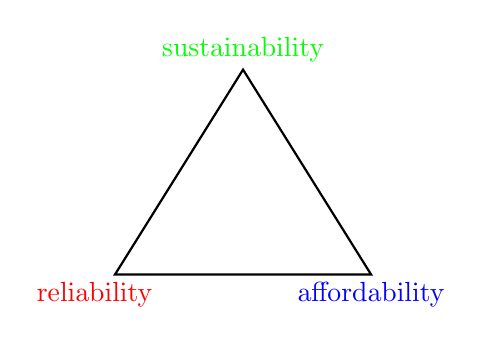
\begin{tikzpicture}[thick,scale=1.3]

      \coordinate (O) at (0,0);
      \coordinate (A) at (2.5,0);
      \coordinate (B) at (1.25,2);
      \draw (O)--(A)--(B)--cycle;
      \draw (1.25,2.2) node[green]{sustainability};
      \draw (-0.2,-0.2) node[red]{reliability};
      \draw (2.5,-0.2) node[blue]{affordability};
  \end{tikzpicture}

  \end{column}


  \begin{column}{8cm}
\begin{itemize}
  \item \alert{Sustainability}: Respect environmental constraints (greenhouse gas emissions, preservation of wildlife), as well as social and political constraints (public acceptance of transmission lines, onshore wind, nuclear power)
  \item \alert{Reliability}: Ensure energy services are delivered whenever needed, even when the wind isn't blowing and the sun isn't shining, and even when components fail
  \item \alert{Affordability}: Deliver energy at a reasonable cost
  \end{itemize}

  \end{column}
\end{columns}


  \vspace{.3cm}

  Some of these policy targets can come into \alert{conflict} - an \alert{energy trilemma} (see EI1).

\end{frame}

\begin{frame}
  \frametitle{Why it's computationally hard: many components and interactions}

  Need to model: (at least) all of Europe for market integration; enough spatial and temporal detail to capture all important effects;
  all interactions between energy sectors; correct physics.

  \vspace{.3cm}

\begin{columns}[T]
  \begin{column}{6cm}

    \vspace{.2cm}
    \centering
    \includegraphics[width=6.5cm]{pypsa-eur-grid.pdf}
  \end{column}

    \begin{column}{5.5cm}

  \centering
  \includegraphics[width=6cm]{20200223_multisector_figure.pdf}
  \end{column}
\end{columns}

\end{frame}


\begin{frame}
  \frametitle{Why it's hard: non-linearities and social effects}

\begin{columns}[T]
  \begin{column}{7.5cm}

    \vspace{.2cm}
    \centering
    \includegraphics[width=8cm]{LCOE-press-release-edited.jpg}
  \end{column}
  \begin{column}{6cm}

\centering
\includegraphics[width=5cm]{nein_zur_monstertrasse}
  \end{column}
\end{columns}
\end{frame}



\begin{frame}
  \frametitle{Not everyone gets it right...}
\begin{columns}[T]
  \begin{column}{7.5cm}

    \vspace{.2cm}
    \centering
    \includegraphics[width=7cm]{2019-01-10-IEEFA-EIA-coal-all-consumption-forecasts-470-x-395-v2-768x646}
  \end{column}
  \begin{column}{7.5cm}

    \vspace{.2cm}
    \centering
    \includegraphics[width=7cm]{auke.jpg}
  \end{column}
\end{columns}
\end{frame}

\begin{frame}
  \frametitle{...and it's not always uncontroversial}

  \begin{columns}[T]
\begin{column}{6cm}
  \includegraphics[trim=0 0cm 0 0cm,width=6cm,clip=true]{sinn-atomkraft}

    {\small Sinn's study was \href{https://doi.org/10.1016/j.euroecorev.2018.07.004}{\bf\color{blue}\underline{debunked}}
       using an
      open model (he exaggerated storage requirements by `up to
      \alert{two orders of magnitude}')}

\end{column}
\begin{column}{6cm}

  \includegraphics[trim=0 0cm 0 0cm,width=5.4cm,clip=true]{sinn-eautos}

  {\small Sinn's study was \href{https://doi.org/10.1016/j.joule.2019.06.002}{\bf\color{blue}\underline{debunked}}, shown to use cherry-picked assumptions}
\end{column}
\end{columns}

\end{frame}



\begin{frame}[fragile]
  \frametitle{What can informatics contribute?}

  Informatics can contribute on the \alert{data side}:
  \begin{itemize}
  \item Processing and analysing enormous weather datasets
  \item Geographical potential analysis with GIS tools
  \item Visualisation of results
  \end{itemize}
  and on the \alert{algorithmic side}:
  \begin{itemize}
  \item New optimization routines for speed and accuracy
  \item Data reduction and feature identification
  \item Information theory to trace interdependencies
  \end{itemize}

  Build on informatics' \alert{interdisciplinary} links to engineering, economics, meteorology, mathematics and physics.
\end{frame}





\begin{frame}
  \frametitle{Course outline}

  This course will cover the following topics:

  \begin{itemize}
  \item General properties of renewable power, time series analysis
    \item Backup generation, curtailment
  \item Network modelling in power systems
  \item Storage modelling
  \item Optimization theory
  \item Energy system economics
      \item Complex network techniques for renewable energy networks (flow tracing, etc.)
    \item Current research topics
  \end{itemize}


\end{frame}






\section{The Greenhouse Gas Challenge}


\begin{frame}
  \frametitle{2015 Paris Agreement}

  The 2015 Paris Agreement pledged its signatories to
 `pursue efforts to limit [global warming above pre-industrial levels] to \alert{1.5$^\circ$C}' and
   hold `the increase...to \alert{well below 2$^\circ$C}'.
  These targets were chosen to avoid potentially irreversible \alert{tipping points} in the Earth's systems.


  \begin{columns}[T]
\begin{column}{9.5cm}

  \includegraphics[width=10cm]{nclimate3013-f1.jpg}
\end{column}
\begin{column}{4.5cm}

  \vspace{.3cm}

  WAIS: West Antarctic Ice Sheet (5m sea level rise)

  \vspace{.2cm}

  Greenland (7m)

  \vspace{.2cm}

  THC: thermohaline circulation (warms Europe)

  \vspace{.2cm}

  ENSO: El Niño–Southern Oscillation (extreme weather)

  \vspace{.2cm}

  EAIS: East Antarctic Ice Sheet ($>50$ m)

\end{column}
  \end{columns}

\source{\href{https://www.nature.com/articles/nclimate3013}{`Why the right climate target was agreed in Paris'}, Nature Climate Change, 2016}
\end{frame}


\begin{frame}
  \frametitle{The Global Carbon Dioxide Challenge: Net-Zero Emissions by 2050}

  \begin{columns}[T]
\begin{column}{7.5cm}

  \includegraphics[width=8cm]{ipcc-sr15}


\end{column}
\begin{column}{6cm}
  \begin{itemize}
\item Scenarios for global CO$_2$ emissions that limit warming to 1.5$^\circ$C about industrial levels (\alert{Paris agreement})
\item Today emissions \alert{still rising}
\item Level of use of negative emission technologies (NET) depends on rate of progress
\item 2$^\circ$C target without NET also needs
  rapid fall by 2050
\item Common theme: \alert{net-zero by 2050}
\end{itemize}
\end{column}
  \end{columns}

    \source{\href{http://ipcc.ch/report/sr15/}{IPCC SR15 on 1.5C, 2018}}
\end{frame}

\begin{frame}
  \frametitle{The Greenhouse Gas Challenge: Net-Zero Emissions by 2050}

  Paris-compliant 1.5$^\circ$~C scenarios from European Commission - \alert{net-zero GHG in EU by 2050}

  \vspace{.4cm}

  %Figure 6 from https://ec.europa.eu/clima/sites/clima/files/docs/pages/com_2018_733_en.pdf
  \includegraphics[width=14cm]{eu-lts-net-zero.png}


    \source{\href{https://ec.europa.eu/clima/sites/clima/files/docs/pages/com_2018_733_en.pdf}{European Commission `Clean Planet for All', 2018}}
\end{frame}


\begin{frame}
  \frametitle{It's not just about electricity demand...}

  %GHG in 2016 are 4.291~Gt, CO2 is 3.489 ~Gt without LULUCF and without indirect
  %Global is 36.2 Gt (EU figure from carbonbrief excludes LULUCF, so assume global also)
%https://www.carbonbrief.org/analysis-global-co2-emissions-set-to-rise-2-percent-in-2017-following-three-year-plateau
  EU28 \co2{} emissions in 2016 (total 3.5~Gt \co2, 9.7\% of global):

  \centering
    % left bottom right top
  \includegraphics[trim=0 0.7cm 0 0.5cm,width=12cm]{EU28-emissions_pie-2016-CO2-190311.pdf}

%  ...\alert{but} wind and solar will dominate primary energy in all sectors, so electrification is critical.

  \source{Brown, data from \href{https://www.eea.europa.eu/data-and-maps/data/national-emissions-reported-to-the-unfccc-and-to-the-eu-greenhouse-gas-monitoring-mechanism-13}{EEA}}
\end{frame}



\begin{frame}
  \frametitle{...but electrification of other sectors is critical for decarbonisation}

\alert{Electrification is essential} to decarbonise sectors such as
transport, heating and industry, since we can use low-emission
electricity from e.g. wind and solar to displace fossil-fuelled
transport with electric vehicles, and fossil-fuelled heating with
electric heat pumps.

Some scenarios show a \alert{doubling or more of electricity demand}.

  \vspace{.7cm}

  \begin{columns}[T]
\begin{column}{6cm}
  \includegraphics[trim=0 0cm 0 0cm,width=6cm,clip=true]{tesla.jpg}
\end{column}
\begin{column}{6cm}

  \includegraphics[trim=0 0cm 0 0cm,width=6cm,clip=true]{640px-Heat_Pump.jpg}
\end{column}
\end{columns}



\source{Tesla; heat pump: \href{https://commons.wikimedia.org/w/index.php?curid=10795550}{Kristoferb at English Wikipedia}}

\end{frame}





\begin{frame}{Efficiency of renewables and sector coupling}


  \includegraphics[width=\linewidth,trim=2.7cm 20cm 3.2cm 1.8cm,clip=true]{./graphics/bmwi-whitepaper-figure_18.pdf}

  \source{\href{https://www.bmwi.de/Redaktion/EN/Publikationen/whitepaper-electricity-market.html}{BMWi White Paper 2015}}
\end{frame}



\begin{frame}[fragile]
  \frametitle{Why focus on wind and solar for electricity generation?}
    \begin{columns}[T]
      \begin{column}{4cm}
        \begin{itemize}
        \item construction and operation have low greenhouse gas emissions
        \item good wind and sun are available in many parts of the world
        \item worldwide potential that exceeds demand by many factors
        \item rapidly falling costs
        \end{itemize}
      \end{column}
      \begin{column}{5cm}
        \includegraphics[trim=0 0cm 0 0cm,width=4.5cm,clip=true]{SolarGIS-Solar-map-Germany-de}
      \end{column}
      \begin{column}{5cm}
        \vspace{.8cm}
        \includegraphics[trim=0 0cm 0 0cm,width=5.5cm,clip=true]{43_Mittlere_Windgeschwindigkeit_100_m_Deutschland}
      \end{column}
    \end{columns}


\end{frame}



\begin{frame}{Worldwide potentials}


    \begin{columns}[T]
      \begin{column}{8.5cm}
  \centering
    \includegraphics[width=8.7cm]{global_potentials.png}

      \end{column}
      \begin{column}{6cm}

    \vspace{.5cm}
        \begin{itemize}
        \item Potentials for wind and solar exceed current demand by many factors (ignoring variability)
        \item Other renewable sources include wave, tidal, geothermal, biomass and hydroelectricity
        \item Uranium depends on the reactor: conventional thermal reactors can extract 50-70 times less than fast breeders
        \end{itemize}
      \end{column}
    \end{columns}

      \source{\href{http://solarmarketpathways.org/wp-content/uploads/2017/08/NSC-Achieving-High-PV-Penetration-160526.pdf}{Perez et al, Applied Policy, 2016}}

\end{frame}

\begin{frame}{Low cost of wind \& solar per MWh in 2017 (NB: ignores variability)}

  LCOE = \alert{Levelised Cost of Energy} = Total Costs $/$ Energy Output
  \centering
  \includegraphics[width=14cm]{lazard-cropped.jpg}

  \source{\href{https://www.lazard.com/perspective/levelized-cost-of-energy-2017/}{Lazard's LCOE Analysis V11}}

\end{frame}





\begin{frame}[fragile]
  \frametitle{Must take account of variability...}


  \includegraphics[width=7cm]{variability-berlin}
\hspace{.2cm}
  \includegraphics[width=6cm]{2015-11-30-0300}
\end{frame}

\begin{frame}[fragile]
  \frametitle{...and social \& political constraints}



\begin{columns}[T]

  \begin{column}{5cm}


\centering
\includegraphics[width=5cm]{nein_zur_monstertrasse}

  \end{column}


  \begin{column}{6.7cm}

    \vspace{.5cm}

    Sustainability doesn't just mean taking account of environmental constraints.

    \vspace{.5cm}

    There are also \alert{social and political constraints},
    particularly for transmission grid and onshore wind
    development.

    \vspace{.5cm}

\includegraphics[width=7cm]{Protestplakat-gegen-den-Bau-von-Windraedern-in-Hamburg-Deutschland.jpg}

  \end{column}

\end{columns}

\end{frame}


\begin{frame}
  \frametitle{Energy Transition: Several changes happening simultaneously}

  \alert{Energiewende}: The Energy Transition, consists of several parts:

  \begin{itemize}
  \item Transition to an energy system with low greenhouse gas emissions
  \item Renewables replace fossil-fuelled generation (and nuclear in some countries)
  \item Increasing integration of international electricity markets
  \item Better integration of transmission constraints in electricity markets
  \item Sector coupling: heating, transport and industry electrify
  \item More decentralised location and ownership in the power sector
  \end{itemize}

\end{frame}


\begin{frame}
  \frametitle{Renewables reached 40\% of gross electricity generation in Germany in 2019}

  \centering
  \includegraphics[width=11cm]{fig2-gross-power-production-germany-1990-2019.png}

\end{frame}






\section{Invitation: Balancing Variable Renewable Energy in Europe}



\begin{frame}[fragile]
  \frametitle{Goals for Energy System Modelling}

  \begin{enumerate}
  \item What \alert{infrastructure} (wind, solar, hydro generators,
    heating/cooling units, storage and networks) does a highly renewable energy system
    require and \alert{where} should it go?
  \item Given a desired \co2 emissions reduction (e.g. 95\% compared to 1990),
    what is the \alert{cost-optimal} combination of infrastructure?
  \item How do we deal with the \alert{variability} of wind and solar: balancing in space with networks or in time with storage?
  \end{enumerate}



\end{frame}


\begin{frame}
  \frametitle{Variability: Single wind site in Berlin}

  Looking at the wind output of a single wind plant over two weeks, it is highly
  variable, frequently dropping close to zero and fluctuating strongly.

  \centering
  \includegraphics[width=12cm]{variability-berlin}


\end{frame}



\begin{frame}
  \frametitle{Electricity consumption is much more regular}

  Electrical demand is much more regular over time - dealing with the
  \alert{mismatch} between locally-produced wind and the demand would
  require a lot of storage...

  \centering
  \includegraphics[width=12cm]{DE-load}


\end{frame}



\begin{frame}
  \frametitle{Variability: Different wind conditions over Germany}

  The wind does not blow the same at every site at every time: at a given time there are a variety of wind conditions across Germany. These differences \alert{balance out over time and space}.

  \centering
  \includegraphics[width=10cm]{2015-05-13-1100}

  \source{\url{https://earth.nullschool.net/}}

\end{frame}




\begin{frame}
  \frametitle{Variability: Single country: Germany}

  For a whole country like Germany this results in valleys and peaks that are  somewhat smoother, but the profile still frequently
  drops close to zero.

  \centering
  \includegraphics[width=12cm]{variability-de}


\end{frame}



\begin{frame}
  \frametitle{Variability: Different wind conditions over Europe}

  The scale of the weather systems are bigger than countries, so to leverage the full smoothing effects, you need to integrate wind at the \alert{continental scale}.

  \centering
  \includegraphics[width=10cm]{2015-11-30-0300}

  \source{\url{https://earth.nullschool.net/}}

\end{frame}



\begin{frame}
  \frametitle{Variability: A continent: Europe}


  If we can integrate the feed-in of wind turbines across the European continent, the
  feed-in is considerably smoother: we've eliminated most valleys and
  peaks.

  \centering
  \includegraphics[width=12cm]{variability-eu}


\end{frame}





\begin{frame}
  \frametitle{Variability: A continent: Wind plus Hydro}

  Flexible, renewable hydroelectricity from storage dams in Scandinavia and the Alps can fill many of the valleys; excess energy can either be curtailed (spilled) or stored.

  \centering
  \includegraphics[width=12cm]{variability-load}


\end{frame}



\begin{frame}
  \frametitle{Daily variations: challenges and solutions}

  \begin{columns}[T]
    \begin{column}{5cm}
      \includegraphics[trim=0 0cm 0 0cm,width=5cm,clip=true]{DE-solar-day.pdf}

      \includegraphics[trim=0 0cm 0 0cm,width=5cm,clip=true]{DE-transport-day.pdf}
    \end{column}
    \begin{column}{4cm}
      \alert{Daily} variations in supply and demand can be balanced by
      \begin{itemize}
      \item \alert{short-term storage} (e.g. batteries, pumped-hydro, small thermal storage)
      \item \alert{demand-side management} (e.g. battery electric vehicles,
        industry)
      \item \alert{east-west grids over multiple time zones}
      \end{itemize}

    \end{column}
    \begin{column}{5cm}
      \includegraphics[trim=0 0cm 0 0cm,width=5cm,clip=true]{pumped-storage-diagram-best1.jpg}

      \vspace{.5cm}

      \includegraphics[trim=0 0cm 0 0cm,width=5cm,clip=true]{tesla-charging.jpg}
    \end{column}
  \end{columns}

\end{frame}




\begin{frame}
  \frametitle{Weekly variations: challenges and solutions}

  \begin{columns}[T]
    \begin{column}{5cm}
      \includegraphics[trim=0 0cm 0 0cm,width=5.3cm,clip=true]{DE-wind-month.pdf}

      \includegraphics[trim=0 0cm 0 0cm,width=5cm,clip=true]{2015-11-30-0300.png}

    \end{column}
    \begin{column}{4cm}
      \href{https://www.youtube.com/watch?v=ttfuEnMz2UM}{\alert{Weekly} variations} in supply and demand can be balanced by
      \begin{itemize}
      \item \alert{medium-term storage} (e.g. chemically with hydrogen or methane storage, thermal energy storage, hydro reservoirs)
      \item \alert{continent-wide grids}
      \end{itemize}

    \end{column}
    \begin{column}{5cm}
      \includegraphics[trim=0 0cm 0 0cm,width=4.5cm,clip=true]{1024px-Gasometer_in_East_London.jpg}

      \includegraphics[trim=0 0cm 0 0cm,width=4.5cm,clip=true]{europe_map.pdf}
    \end{column}
  \end{columns}

\end{frame}




\begin{frame}
  \frametitle{Seasonal variations: challenges and solutions}

  \begin{columns}[T]
    \begin{column}{5cm}
      \includegraphics[trim=0 0cm 0 0cm,width=5cm,clip=true]{DE-wind-solar-year.pdf}

      \includegraphics[trim=0 0cm 0 0cm,width=5cm,clip=true]{DE-heat-year.pdf}
    \end{column}
    \begin{column}{4cm}
      \alert{Seasonal} variations in supply and demand can be balanced by
      \begin{itemize}
      \item \alert{long-term storage} (e.g. chemically with hydrogen or methane storage, long-term thermal energy storage, hydro reservoirs)
      \item \alert{north-south grids over multiple latitudes}
      \end{itemize}

    \end{column}
    \begin{column}{5cm}
      \includegraphics[trim=0 0cm 0 0cm,width=4.7cm,clip=true]{1024px-Gasometer_in_East_London.jpg}

      \vspace{.2cm}

      \includegraphics[trim=0 0cm 0 0cm,width=4.7cm,clip=true]{pit-zoom.png}
    \end{column}
  \end{columns}

\end{frame}



\begin{frame}
  \frametitle{Research approach}

  Avoid too many assumptions. Fix the \alert{boundary conditions}:

  \begin{itemize}
  \item Meet demand for energy services
  \item Reduce \co2 emissions
  \item Conservative predictions for cost developments
  \item No/minimal/optimal grid expansion
  \end{itemize}

  Then \alert{let the math decide the rest}, i.e. choose the number of
  wind turbines / solar panels / storage units / transmission lines to
  minimise total costs (investment \alert{and} operation).

  \vspace{.3cm}

  Generation, storage and transmission optimised \alert{jointly}
  because they are \alert{strongly interacting}.
\end{frame}




\begin{frame}
  \frametitle{Determine optimal electricity system}


\begin{columns}[T]
\begin{column}{7cm}
  \begin{itemize}
  \item Meet all electricity demand.
  \item Reduce \co2{} by 95\% compared to 1990.
  \item \alert{Generation} (where potentials allow): onshore and offshore
    wind, solar, hydroelectricity, backup from natural gas.
  \item \alert{Storage}: batteries for short term, electrolyse hydrogen gas for long term.
  \item \alert{Grid expansion}: simulate everything from no grid expansion (like a \alert{decentralised solution}) to optimal grid expansion (with significant \alert{cross-border trade}).
  \end{itemize}
\end{column}
\begin{column}{6.5cm}


  \vspace{0.3cm}
\centering

\includegraphics[width=7cm]{europe_map}

\end{column}
\end{columns}


\source{PyPSA-Eur, based on ENTSO-E map}
\end{frame}



\begin{frame}[fragile]
  \frametitle{Linear optimisation of annual system costs}

Find the long-term cost-optimal energy system, including investments and short-term costs:
\begin{equation*}
  \textrm{Minimise} \left(\parbox{6em}{\centering\alert{Yearly\\system costs}}\right) = \sum_n \left(\parbox{6em}{\centering\alert{Annualised capital costs}}\right) + \sum_{n,t} \left(\parbox{5em}{\centering\alert{Marginal costs}}\right)
\end{equation*}
subject to
\begin{itemize}
\item meeting \alert{energy demand} at each node $n$ (e.g. region) and time $t$ (e.g. hour of year)
\item wind, solar, hydro (variable renewables) \alert{availability time series} $\forall\: n,t$
\item \alert{transmission constraints} between nodes, \alert{linearised power flow}
\item (installed capacity) $\leq$ (\alert{geographical potentials} for renewables)
\item \alert{CO${}_2$ constraint} (e.g. 95\% reduction compared to 1990)
\end{itemize}

In short: mostly-greenfield investment optimisation, multi-period with linear power flow.

Optimise transmission, generation and storage \alert{jointly}, since they're strongly interacting.
\end{frame}





\begin{frame}
  \frametitle{Optimization problem}

This has the general form of an \alert{optimization problem} for which there are specialized algorithms. For \alert{continuous linear problems} these solve in \alert{polynomial time}.

We have an \alert{objective function} $f: \R^k \to \R$ which is to be either maximised or minimised:
\begin{equation*}
  \max_{x} f(x)
\end{equation*}
[$x = (x_1, \dots x_k)$] subject to some \alert{constraints} within $\R^k$:
\begin{align*}
  g_i(x) & = c_i \hspace{1cm}\leftrightarrow\hspace{1cm} \l_i \hspace{1cm} i = 1,\dots n \\
  h_j(x) & \leq d_j \hspace{1cm}\leftrightarrow\hspace{1cm} \m_j \hspace{1cm} j = 1,\dots m
\end{align*}


The constraints define a \alert{feasible space} within $\R^k$.


We introduce KKT multipliers $\l_i$ and $\m_j$ for each constraint
equation, which have an economic interpretation as the \alert{shadow
  prices} of the constraints. They tell us how the value
of the objective function $f(x^*)$ changes as we relax/tighten the
corresponding constraints.

\end{frame}




\begin{frame}
  \frametitle{Linear optimisation problem}


  Objective is the minimisation of \alert{total annual system costs}, composed of \alert{capital costs} $c_*$ (investment costs) and \alert{operating costs} $o_*$ (fuel ,etc.):
  \begin{equation*}
\min    f(F_\ell, f_{\ell,t}, G_{i,s},  g_{i,s,t}) =  \sum_{\ell} c_l F_\ell + \sum_{i,s} c_{i,s} G_{i,s} + \sum_{i,s,t} w_t o_{i,s} g_{i,s,t}
  \end{equation*}
  We optimise for $i$ nodes, representative times $t$ and transmission lines $l$:
  \begin{itemize}
  \item the transmission capacity $F_\ell$ of all the lines $\ell$
  \item the flows $f_{\ell,t}$ on each line $\ell$ at each time $t$
  \item the generation and storage capacities $G_{i,s}$ of all technologies (wind/solar/gas etc.) $s$ at each node $i$
  \item the dispatch $g_{i,s,t}$ of each generator and storage unit at each point in time $t$
  \end{itemize}

  Representative time points are weighted $w_t$ such that $\sum_t w_t = 365*24$ and the capital costs $c_*$ are annualised, so that the objective function represents the annual system cost.

\end{frame}



\begin{frame}
  \frametitle{Constraints 1/6: Nodal energy balance}

  Demand $d_{i,t}$ at each node $i$ and time $t$ is always met by
  generation/storage units $g_{i,s,t}$ at the node or from transmission
  flows $f_{\ell,t}$ on lines attached at the node (Kirchhoff's Current Law):
    \begin{equation*}
      \sum_{s} g_{i,s,t} - d_{i,t} =  \sum_{\ell } K_{i\ell} f_{\ell,t}  \hspace{1cm}\leftrightarrow\hspace{1cm} \l_{i,t}
    \end{equation*}

    Nodes are shown as thick busbars connected by transmission lines (thin lines):

\centering
\begin{circuitikz}
  \draw (1.5,14.5) to [short,i^=$f_1$] (1.5,13);
  \draw [ultra thick] (0,13) node[anchor=south]{i} -- (4,13);
  \draw(2.5,13) |- +(0,0.5) to [short,i^=$f_2$] +(5,0.5) |- +(0,-0.5);
  \draw [ultra thick] (6,13) node[anchor=south]{j} -- +(4,0);
  \draw (8.5,14.5) to [short,i^=$f_3$] +(0,-1.5);
  \draw (0,-0.5) ;
  \draw (0.5,13) -- +(0,-0.5) node[sground]{};
  \draw (2,12) node[vsourcesinshape, rotate=270](V2){}
  (V2.left) -- +(0,0.6);
  \draw (3.5,12) node[vsourcesinshape, rotate=270](V2){}
  (V2.left) -- +(0,0.6);
  \draw (0.5,11) node{$d_i$};
  \draw (2,11) node{$g_{i,w}$};
  \draw (3.5,11) node{$g_{i,s}$};
  \draw (2,10.3) node{$ g_{i,w} + g_{i,s} - d_i = f_2 -f_1$};
  \draw (6.5,13) -- +(0,-0.5) node[sground]{};
  \draw (8,12) node[vsourcesinshape, rotate=270](V2){}
  (V2.left) -- +(0,0.6);
  \draw (9.5,12) node[vsourcesinshape, rotate=270](V2){}
  (V2.left) -- +(0,0.6);
  \draw (6.5,11) node{$d_j$};
  \draw (8,11) node{$g_{j,w}$};
  \draw (9.5,11) node{$g_{j,s}$};
  \draw (8,10.3) node{$ g_{j,w} + g_{j,s} - d_{j} = -f_2 - f_3$};

\end{circuitikz}


\end{frame}



\begin{frame}
  \frametitle{Constraints 2/6: Generation availability}
  Generator/storage dispatch $g_{i,s,t}$ cannot exceed availability $G_{i,s,t}*G_{i,s}$, made up of per unit availability $0 \leq G_{i,s,t} \leq 1$ multiplied by the capacity $G_{i,s}$. The capacity is bounded by the installable potential $\hat{G}_{i,s}$.
    \begin{equation*}
      0 \leq g_{i,s,t} \leq G_{i,s,t}* G_{i,s} \leq  G_{i,s} \leq  \hat{G}_{i,s}
    \end{equation*}

    \centering
      \includegraphics[width=11cm]{scigrid-curtailment}

\end{frame}




\begin{frame}
  \frametitle{Installation potentials limited by geography}

  Expansion potentials are limited by \alert{land usage} and
  \alert{conservation areas}; potential yearly energy yield at each site
  limited by \alert{weather conditions}:

  \centering
  \includegraphics[width=14.5cm]{average_power_density_potential-eps-converted-to.pdf}
\end{frame}




\begin{frame}
  \frametitle{Constraints 3/6: Storage consistency}

  Storage units such as batteries or hydrogen storage can work in both
  storage and dispatch mode. This has to be consistent with the state
  of charge $e_{i,s,t}$:
  \begin{align*}
    e_{i,s,t} = \eta_0e_{i,s,t-1} + \eta_1g_{i,s,t,\textrm{store}} -  \eta_2^{-1} g_{i,s,t,\textrm{dispatch}}
  \end{align*}

  The state of charge is limited by the energy capacity $E_{i,s}$:
  \begin{align*}
    0 \leq e_{i,s,t} \leq E_{i,s} \quad \forall i,s,t
  \end{align*}


  There are efficiency losses $\eta$; hydroelectric dams can also have a river inflow.

\end{frame}




\begin{frame}
  \frametitle{Constraints 4/6: Kirchoff's Laws for Physical Flow}

  The linearised \alert{power flows} $f_\ell$ for each line $\ell \in
  \{1,\dots L\}$ in an AC network are determined by the
  \alert{reactances} $x_\ell$ of the transmission lines and the
  \alert{net power injection} at each node $p_i$ for $i\in\{1,\dots
  N\}$.


  We have to satisfy Kirchoff's Laws, which can be compactly expressed
  using the \alert{incidence matrix} $K \in \R^{N\times L}$ (boundary
  operator in homology theory) of the graph and the \alert{cycle
    basis} $C \in \R^{L\times(L-N+1)}$ (kernel of $K$)

  \begin{itemize}
  \item  Kirchoff's Current Law: $p_i = \sum_{\ell} K_{i\ell} f_\ell$
  \item  Kirchoff's Voltage Law: $\sum_\ell C_{\ell c} x_\ell f_\ell = 0$
  \end{itemize}

\end{frame}



\begin{frame}
  \frametitle{Constraints 5/6: Transmission Line Thermal Limits}

    Transmission flows cannot exceed the thermal capacities of the transmission lines (otherwise they sag and hit buildings/trees):
    \begin{equation*}
      | f_{\ell,t} | \leq  F_\ell
    \end{equation*}

\end{frame}



\begin{frame}
  \frametitle{Constraints 6/6: Global constraints on \co2 and transmission volumes}
  CO${}_2$ limits are respected, given emissions $\varepsilon_{i,s}$ for each fuel source $s$:
    \begin{equation*}
      \sum_{i,s,t}  g_{i,s,t} \frac{\varepsilon_{i,s}}{\eta_{s}} \leq \textrm{CAP}_{\textrm{CO}_2} \hspace{1cm} \leftrightarrow \hspace{1cm} \m_{\textrm{CO}_2}
    \end{equation*}
    We enforce a reduction of \co2 emissions by 95\% compared to 1990
    levels, in line with German and EU targets for 2050.

    Transmission volume limits are respected, given length $d_\ell$ and capacity $F_\ell$ of each line:
    \begin{equation*}
      \sum_{\ell} d_\ell   F_\ell \leq \textrm{CAP}_{\textrm{trans}} \hspace{1cm} \leftrightarrow \hspace{1cm} \m_{\textrm{trans}}
    \end{equation*}
    We  successively change the transmission limit, to assess the costs of balancing power in time (i.e. storage) versus space (i.e. transmission networks).

\end{frame}



\begin{frame}
\frametitle{Model Inputs and Outputs}

\begin{columns}
  \begin{column}{6cm}


    \begin{table}[!t]
	\centering
	\begin{tabular}{@{}p{1.15cm}p{4.54cm}@{}}
\toprule
\alert{Inputs} & Description \\
\midrule
$d_{i,t}$ & Demand (inelastic) \\
$G_{i,s,t}$ & Per unit availability for wind and solar \\
$\hat{G}_{i,s}$ & Generator installable potentials \\
various & Existing hydro data \\
various & Grid topology \\
$\eta_*$ & Storage efficiencies \\
$c_{i,s}$ & Generator capital costs \\
$o_{i,s,t}$ & Generator marginal costs \\
$c_\ell$ & Line costs \\
\bottomrule
	\end{tabular}
\end{table}
  \end{column}
    \begin{column}{1cm}


      \vspace{1cm}

      $\to$

    \end{column}
  \begin{column}{6cm}


    \begin{table}[!t]
	\centering
	\begin{tabular}{@{}p{1.15cm}p{4.54cm}@{}}
\toprule
\alert{Outputs} & Description \\
\midrule
$G_{i,s}$ &  Generator capacities \\
$g_{i,s,t}$ & Generator dispatch \\
$F_\ell$ & Line capacities \\
$f_{\ell,t}$ & Line flows \\
$\lambda_*,\mu_*$ & Lagrange/KKT multipliers of all constraints \\
f & Total system costs \\
\bottomrule
	\end{tabular}
\end{table}
  \end{column}

\end{columns}
\end{frame}




\begin{frame}
  \frametitle{Costs and assumptions for the electricity sector (projections for 2030)}

  \begin{table}
\centering
\begin{tabular}{@{}lrlrr@{}}
\toprule
Quantity                &Overnight  Cost [\euro]  &Unit & FOM [\%/a] & Lifetime [a] \\
\midrule
Wind onshore    &1182   &kW\el &3 & 20   \\
Wind offshore  &2506   &kW\el  &3& 20  \\
Solar PV           &600   &kW\el &4 & 20   \\
Gas             &400    &kW\el  &4& 30  \\
%Gas marginal            &75     &\euro{}/MWh$_{\textrm{e}}$    \\
Battery storage         &1275   &kW\el  & 3 & 20 \\
Hydrogen storage        &2070   &kW\el  & 1.7 &20 \\
Transmission line       &400    &MWkm & 2 & 40\\
\bottomrule
\end{tabular}
\end{table}
  Interest rate of 7\%, storage efficiency losses, only gas has \co2 emissions, gas marginal costs.

  Batteries can store for 6 hours at maximal rating (efficiency $0.9\times 0.9$), hydrogen storage for 168 hours (efficiency $0.75\times 0.58$).
\end{frame}





\begin{frame}
  \frametitle{Costs: No interconnecting transmission allowed}



\begin{columns}[T]
  \begin{column}{4.9cm}

  Technology~by~energy:
  % left bottom right top
  \begin{tabular}{cc}
    \includegraphics[trim=0 0cm 0 0cm,width=3.2cm,clip=true]{total-pie-0-0} &
  \end{tabular}


  Average~cost~\alert{\euro 86/MWh}:

  \includegraphics[width=3.6cm]{total-costs-joint-1}

  \end{column}

  \begin{column}{9cm}
    % left bottom right top
    \centering
    \includegraphics[trim=0 4cm 0 4cm,width=8cm,clip=true]{euro-pie-0-0}

    \raggedright
    Countries must be self-sufficient at all times; lots of storage and some gas to deal with fluctuations of wind and solar.
  \end{column}

\end{columns}
\end{frame}


\begin{frame}
  \frametitle{Dispatch with no interconnecting transmission}

  For Great Britain with no interconnecting transmission, excess wind is either stored as hydrogen or curtailed:

  \centering
  \includegraphics[width=13cm]{GB-0}
\end{frame}


\begin{frame}
  \frametitle{Costs: Cost-optimal expansion of interconnecting transmission}


\begin{columns}[T]
  \begin{column}{5.3cm}

  Technology~by~energy:
  % left bottom right top
    \begin{tabular}{cc}
    \includegraphics[trim=0 0cm 0 0cm,width=3.2cm,clip=true]{total-pie-0-5} &
  \end{tabular}

  Average~cost~\alert{\euro 64/MWh}:

  \includegraphics[width=4.7cm]{total-costs-joint-2}

  \end{column}

  \begin{column}{9cm}
    % left bottom right top
    \centering
    \includegraphics[trim=0 4cm 0 4cm,width=8cm,clip=true]{euro-pie-0-5}

    \raggedright
    Large transmission expansion; onshore wind dominates. This optimal solution may run into public acceptance problems.
  \end{column}


\end{columns}

\end{frame}


\begin{frame}
  \frametitle{Dispatch with cost-optimal interconnecting transmission}

  Almost all excess wind can be now be exported:

  \centering
  \includegraphics[width=13cm]{GB-1}
\end{frame}



\begin{frame}
  \frametitle{Electricity Only Costs Comparison}

\begin{columns}[T]
  \begin{column}{9cm}

    \vspace{0.5cm}
  \includegraphics[width=9cm]{opteu_paper2-elec_only-costs-curve}

  \end{column}

  \begin{column}{5cm}
    \begin{itemize}
    \item Average total system costs can be as low as \euro~64/MWh
     \item Energy is dominated by wind (64\% for the cost-optimal system), followed
       by hydro (15\%) and solar (17\%)
     \item Restricting transmission results in more storage to deal with variability, driving up the costs by up to 34\%
     \item Many benefits already locked in at a few multiples of today's grid
    \end{itemize}

  \end{column}

\end{columns}
\end{frame}



\begin{frame}
  \frametitle{Different flexibility options have difference temporal scales}

\begin{columns}[T]
  \begin{column}{10.5cm}

    \vspace{0.5cm}
  \includegraphics[width=11cm]{soc_series_LV0-25_H2_hydro_diw2030_solar1_7-eps-converted-to.pdf}

  \end{column}

  \begin{column}{3cm}
    \vspace{1cm}
    \begin{itemize}
    \item Hydro reservoirs are \alert{seasonal}
    \item Hydrogen storage is \alert{multi-weekly}
    \end{itemize}

  \end{column}

\end{columns}
\end{frame}



\begin{frame}
  \frametitle{Different flexibility options have difference temporal scales}

\begin{columns}[T]
  \begin{column}{10.5cm}

    \vspace{0.5cm}
  \includegraphics[width=11cm]{soc_series_LV0-25_all_2011-08_diw2030_solar1_7-eps-converted-to.pdf}

  \end{column}

  \begin{column}{3cm}
        \vspace{2cm}
    \begin{itemize}
    \item Pumped hydro and battery storage are \alert{daily}
    \end{itemize}

  \end{column}

\end{columns}
\end{frame}


\begin{frame}
  \frametitle{Features of this example}

  This example has several features which will accompany us through the lecture course:
  \begin{enumerate}
  \item We have to account for the variations of wind and solar in \alert{time} and \alert{space}.
  \item These variations take place at \alert{different scales} (daily, multi-week, seasonal).
  \item We often have a choice between balancing in \alert{time} (with storage) or in \alert{space} (with networks).
  \item Optimisation is important to increase cost-effectiveness, but
    we should also look at \alert{near-optimal} solutions.
  \end{enumerate}

  \vspace{1cm}
  Full paper reference: D. Schlachtberger, T. Brown, S. Schramm, M. Greiner, ``The Benefits of Cooperation in a Highly Renewable European Electricity Network'', Energy, 134, 469-481, 2017, \href{https://arxiv.org/abs/1704.05492}{arXiv:1704.05492}.
\end{frame}

\end{document}
